% A skeleton file for producing Computer Engineering reports
% https://kgcoe-git.rit.edu/jgm6496/KGCOEReport_template

\documentclass[CMPE]{../KGCOEReport}

% The following should be changed to represent your personal information
\newcommand{\classCode}{CMPE 460}  % 4 char code with number
\newcommand{\name}{Andrei Tumbar}
\newcommand{\LabSectionNum}{2}
\newcommand{\LabInstructor}{Beato}
\newcommand{\TAs}{Xavier Brooks\\
Diana Yakobchuk\\
Charles Poliwoda}
\newcommand{\exerciseNumber}{4}
\newcommand{\exerciseDescription}{Bluetooth \& I2C}
\newcommand{\dateDone}{2/4/2022}
\newcommand{\dateSubmitted}{2/11/2022}
\newcommand{\LectureSectionNum}{1}
\newcommand{\LectureInstructor}{Beato}

\usepackage{tikz}
\usepackage{circuitikz}
\usetikzlibrary{calc}
\usepackage{multirow}
\usepackage{titlesec}
\usepackage{float}
\usepackage{lmodern}
\usepackage{pgfplots}
\usepackage{siunitx}
\usepackage{subcaption}
\usepackage{graphicx}
\usepackage[usestackEOL]{stackengine}
\usepackage{scalerel}
\usepackage[T1]{fontenc}
\usepackage{amsmath}
\usepackage{pdfpages}


\def\code#1{\texttt{#1}}

\begin{document}
    \maketitle
    \section*{Description}

   	This exercise consisted of two parts, configuring a bluetooth peripheral to work over
   	external UART pin and configuring I2C to drive an OLED display. The bluetooth portion
   	of the lab worked by connecting a smart phone to the bluetooth device and creating
   	simple communication link between the phone and the UART displayed over USB. The
   	purpose in this exercise was to create a simple method of wireless communication and
   	control so that we may debug/control our boards without need to be directly linked to
   	USB. The second portion of the exercise involved writing a driver to control on OLED
   	display. The OLED display is to be used later to view the camera data, however it can
   	also display text and arbitrary imagery.

    \section*{Code description}
    \subsection*{Bluetooth}

    The design of the bluetooth UART device had identical initialization to that of
    the USB UART. A library was written to provide a generic init/read/write interface
    between any of the UART compatible devices. The same set of functions is used and
    simply passing a certain ID will select which device to read, write or initialize.
    This allowed the same code to be used from lab2 for both the bluetooth and USB UART
    peripherals which sped up the development process.\\

	The implementation for the chatroom was simple. Both the bluetooth and the USB devices
	were polled for input data. When data from one of the devices was received, it was
	then transmitted to the other device. The public facing interface to UART for
	both devices is completely abstracted from the specific features of the MSP432
	board and therefore allows for adaptation to other boards if the future need arises.

	\begin{figure}[ht]
	\begin{subfigure}{.5\textwidth}
	  \centering
	  % include first image
	  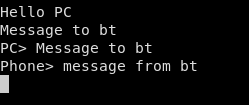
\includegraphics[width=.8\linewidth]{chatroom_pc}
	  \caption{Screenshot of chatroom from PC end.}
	  \label{fig:sub-first}
	\end{subfigure}
	\begin{subfigure}{.4\textwidth}
	  \centering
	  % include second image
	  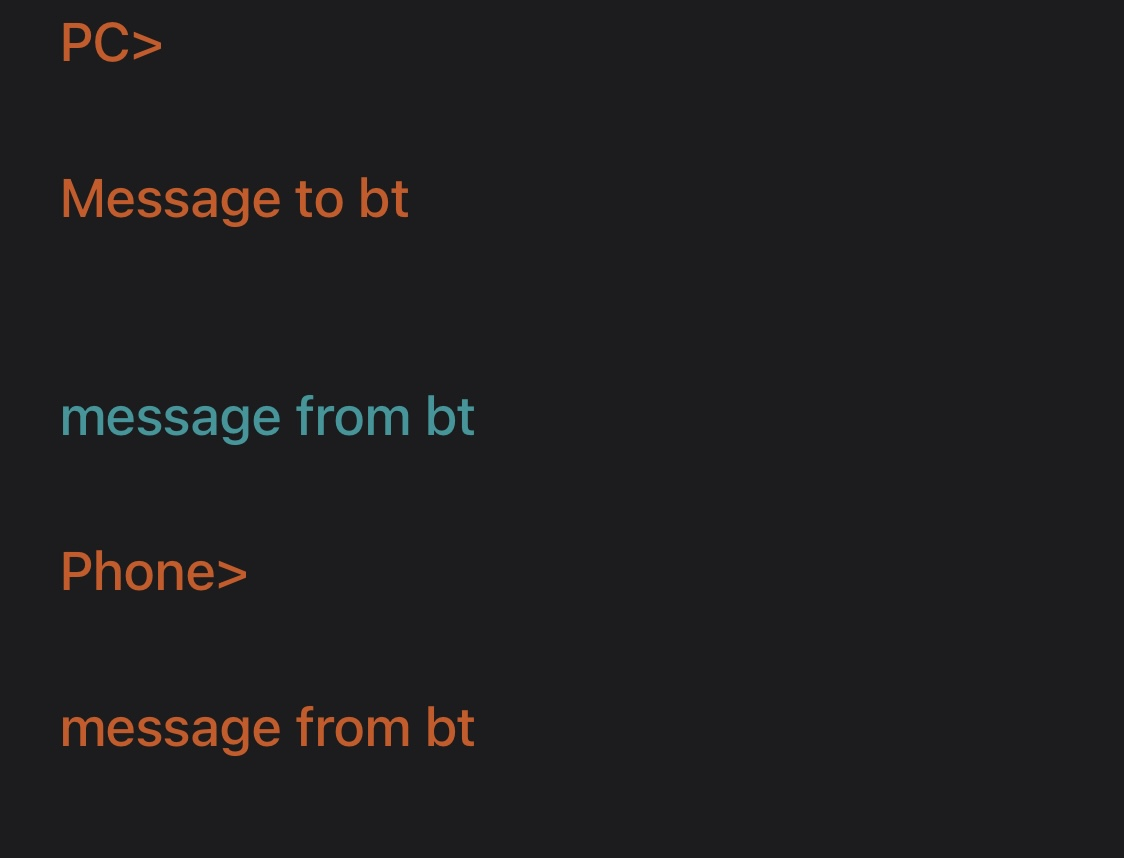
\includegraphics[width=.8\linewidth]{chatroom_bt}
	  \caption{Screenshot of chatroom from phone/bluetooth end.}
	  \label{fig:sub-second}
	\end{subfigure}
	\caption{Screen captures of chatroom in operation on both sides of the comm-link}
	\label{fig:p21}
	\end{figure}

	Figure \ref{fig:p21} shows the operation of the chatroom from both sides of the
	comm-link. We can see the correct operation of the bluetooth-usb chatroom.

	\subsection*{I2C OLED}

	The OLED display is a simple display that communicates with a master device over
	an I2C link. The I2C initialization was fairly straight forward. The UART code was
	similar in that same polling model was used to operate the I2C peripheral. The next
	layer above the I2C driver involved abstracting out the canvas that was used to draw
	on the OLED screen. The public facing interface of the OLED driver allowed the user to
	print text on a canvas or to manually draw directly to this canvas. The canvas could
	then be written via I2C to the OLED display. This design allows for high amounts of
	flexibility in the future as well as hiding the inner workings of the OLED and I2C
	drivers in lower levels of the program.\\

	An image was taken of the OLED displaying text where each line is written separately
	to the display.

	\begin{figure}[ht]
	  \centering
	  % include first image
	  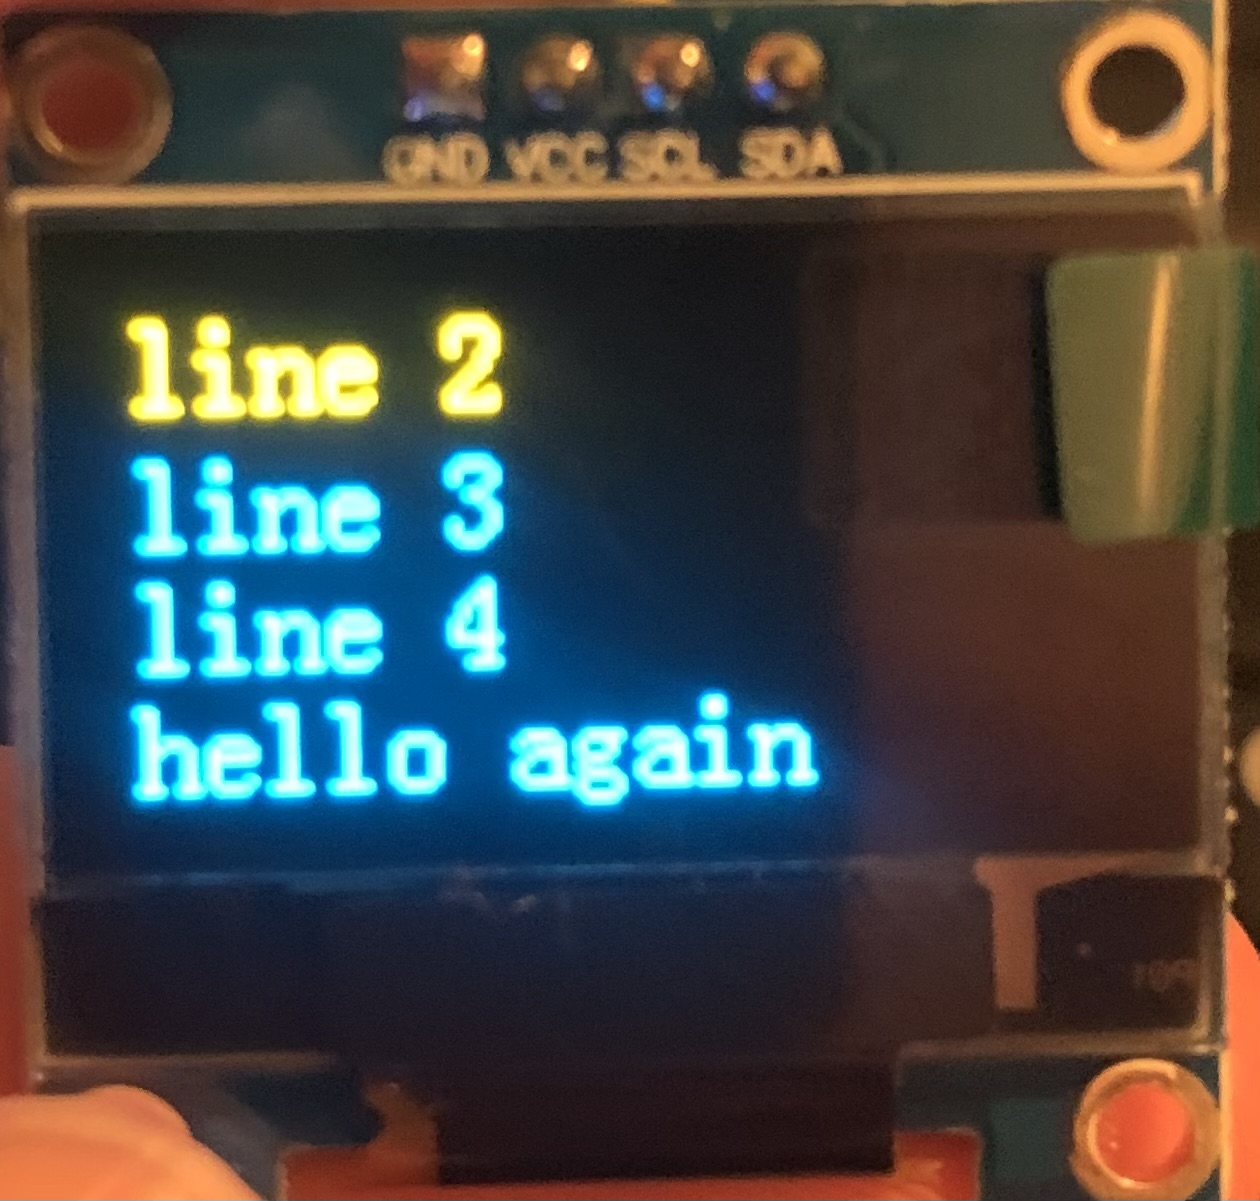
\includegraphics[width=.4\linewidth]{i2c}
	  \caption{OLED screen with text.}
	  \label{fig:oled}
	\end{figure}

	We can see in Figure \ref{fig:oled} the correct operation of the text rendering
	operated by the OLED driver. A total of five lines were printed to the OLED display.
	We can see from the figure that the first line is no longer shown as the text canvas
	scrolled up when the display was filled.

	\section*{Bluetooth question}

	Simultaneous input is handled in the main loop by polling each UART device in a
	non-blocking manner. This means that we simply check if data is available and if
	not, we check the next UART device.

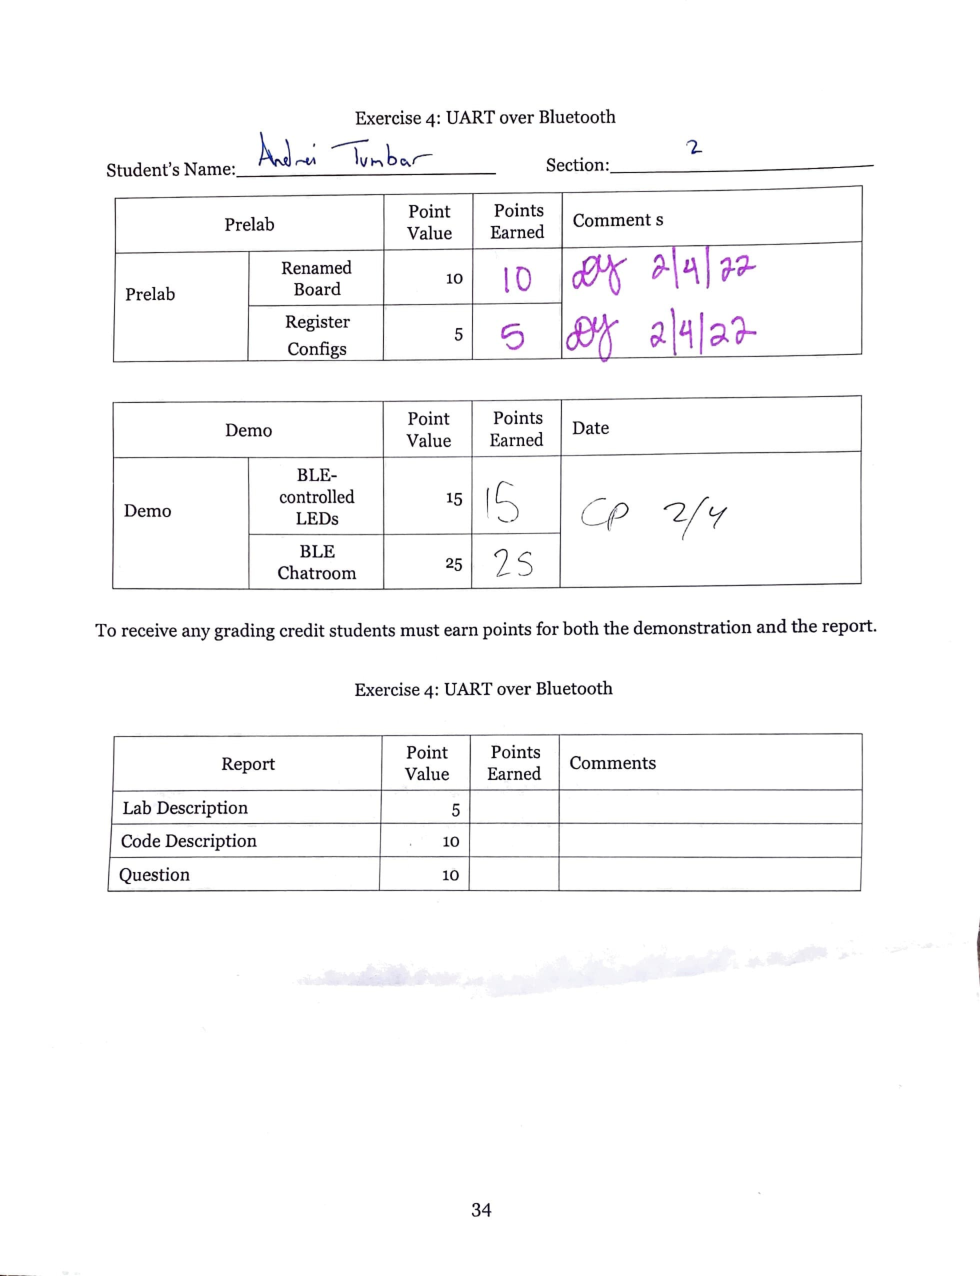
\includepdf[pages=-,pagecommand={},width=\textwidth]{signoff4.pdf}

\end{document}
